% !TeX encoding=utf8
% !TeX spellcheck = de-CH

\chapter{Analyse}
%TODO: Abgleich mit: http://www.ptb.de/cms/fileadmin/internet/fachabteilungen/abteilung_4/4.4_zeit_und_frequenz/4.42/dcf77.pdf

%TODO: PTB-Doku: Kapitel 4.3 (Phasenmodulation)? / 6.1 / 7.3.3 / 7.3.1 / 7.3.2?


\section{Allgemein}
Wieso braucht es Zeitsynchronisation? Was für Probleme und Schwierigkeiten können dabei auftreten? Diese Fragen aus der Aufgabenstellung werden in den nachfolgenden Kapiteln detailliert beantwortet.

\subsection{Hintergründe} \label{subsec:Analyse:Hintergruende}
In der heutigen Zeit sind wir es uns gewohnt, dass wir uns darauf verlassen können, dass unsere Uhren die gleiche, oder zumindest beinahe die gleiche, Zeit anzeigen. 
Wie war das früher? Heute würde vieles nicht mehr funktionieren, wenn wir keine Uhren hätten, bzw. die Uhren nicht synchronisiert werden, oder etwa doch?

\subsubsection{Kurzer Rückblick in die Geschichte} \label{subsubsec:Analyse:BlickGeschichte}
Seit langem ist die Menschheit an der Messung der Zeit, bzw. der Uhrzeit, intressiert.
Seit dem Jahr 300 v. Chr., als die Sonnenuhr in Ägypten erfunden wurde, ergab es sich, dass an zentralen Plätzen solche Sonnenuhren aufgebaut wurden. Wollte man die Uhrzeit wissen, musste man den Weg zur Uhr in Kauf nehmen.
Da die Uhrzeit mit Hilfe des Sonnenstandes ermittelt wurde, gab es Abweichungen zwischen der gemessenen Zeit an verschiedenen Orten. Aufgrund dessen war es damals nicht möglich eine einheitliche Zeit für ein ganzes Reich oder Land zu bestimmen. Die Uhrzeit war jeweils nur lokal pro Stadt oder Gebiet relativ einheitlich.

Im Jahr 1248 wurde die erste mechanische Uhr in Exeter (England) in Betrieb genommen. Sie hatte eine Genauigkeit von einer Stunde und musste täglich mit Hilfe der Sonne kalibriert werden.
Da grosses Interesse an der Uhrzeit bestand, verbreiteten sie sich relativ rasch.
Man konnte sich die Uhrzeit abonnieren, das hiess, einmal am Tag kam jemand vorbei und teilte einem die aktuelle Uhrzeit mit, welche von einer mobilen Uhr abgelesen wurde.

1656 wurde die erste Pendeluhr entwickelt. 1680 war sie so ausgereift, dass sie einen Minutenzeiger erhielt. Das Problem dieser Technologie war, dass eine Pendeluhr nur an ruhigen Standorten funktionierte.
Dies stellte besonders für die Schiffsfahrt eine Problem dar, denn auf See wurde die Uhrzeit zur Berechnung der aktuellen Position verwendet.
Ein Fehler von 4 Sekunden entspricht bereits einer Ungenauigkeit  von rund 1.8 km.
Dies führte dazu, dass die britische Regierung, für eine Genauigkeit von vier Minuten, ein Preisgeld offerierte. Dies entsprach einer Ortungsgenauigkeit von ungefähr 100 km.
John Harrison gelang es 1778 einen Chronometer (H4)\footnote{Die Bezeichnung Chronometer (altgriechisch für "`Zeit"' und "`Mass, Massstab"') steht für besonders präzise Uhren, welche früher zur Zeitbestimmung und zur Navigation auf Schiffen und Flugzeugen benötigt wurden.} zu entwickeln, der diese Ansprüchen erfüllte.
%TODO: Müssen wir evtl. noch kurz erklären / erwähnen was ein Chronometer ist? - SOLVED
%QUELLE: http://de.wikipedia.org/wiki/Chronometer

Bis ins Jahr 1835 wurde die Zeitübermittlung durch akustische oder optische Signale ermöglicht.
Mit dem Aufkommen der Eisenbahn und der somit verbundenen Anforderung, über grössere Strecke die gleiche Zeit zu halten, etablierte sich der Abgleich via elektronische Leitung.

Die ersten Gehversuche der drahtlosen Zeitübermittlung wurden im Jahr 1903 in Washington am United States Naval Observatory gemacht.
Für die Seefahrt startete 1904 die erste regelmässige Zeitübermittlung via Funk. Sechs Jahre später wurde das erste Signal fürs Land, via Eiffelturm, versendet. Im Jahr 1917 hat der erste Vorläufer der heutigen Zeitzeichensender den Betrieb aufgenommen. Die Grosssendestelle Nauen (Bundesland Brandenburg DE) sendete zweimal im Tag via Langwelle ein Zeizeichen. Daraufhin entstand im Laufe der Jahre ein weltweites Netz von Zeitzeichensendern.

Erst im Jahr 1970 wurde der heutige Zeitübermittlungs-Dienst DCF77, in Mainflingen bei Frankfurt in Betrieb genommen.
Kurz darauf, im Jahr 1978, wurden der Betrieb des ersten GPS-Satelliten, mit einer eigenen Atomuhr an Board gestartet.

% http://www.astro-siggi.de/tutorial-funkuhr.html -> astrosiggiFunk
% http://de.wikipedia.org/wiki/Geschichtliche_Entwicklung_der_Zeit%C3%BCbertragung_per_Funk -> wikiFunkHistory
% http://en.wikipedia.org/wiki/Time_signal -> wikiTimeSignal
% http://de.wikipedia.org/wiki/Sonnenuhr -> wikiSunclock

% \subsubsection{Was wäre wenn...}
% Im Kapitel \nameref{subsubsec:Analyse:BlickGeschichte} wurde bereits einige Bereiche genannt wo ein einheitliche und exakte Zeit notwendig ist (z.B. Positionsbestimmung).
%TODO: Dani / Michi - mh: lassen das mal weg. Wäre zwar einen guten Einstieg - SOLVED
%Stichwort: GPS, Börse, ÖV, 
%Heute ist Zeit kostbar -> Auswirkungen enorm (zu spät kommen, etc...)

% \subsection{Was für Schwierigkeiten können dabei auftreten?}
%TODO: Michi: Ich denke wie können dass lassen. Zwar interessanter Artikel, aber nicht wirklich was mit unserer Arbeit zu tun. Wir haben schon sehr viele Infos (meine dies vorallem auf den Artikel bezogen) -> http://diepresse.com/home/spectrum/zeichenderzeit/695559/Auf-der-Hohe-der-Zeit
%TODO: Dani: En Teil chömmer evtl. is Fazit neh, denke münd schono irgendwo ha wo d Schwirigkeite / Problem sind und wases für euses Projekt bedütet. - Ist dies im Fazit? - Pendent

\subsection{Atomuhr}
%http://www.meinberg.de/german/info/atomic_clock.htm
Unter Atomuhr versteht wird folgendes bezeichnet:
\begin{quote}
Eine Atomuhr ist ein Zeitmesser, dessen Zeitnormal die hochfrequente Schwingungsdauer bestimmter Atome ist (z.B. Caesium, Rubidium), die durch ein elektromagnetisches Feld oder optisches Pumpen zu Schwingungen angeregt werden und einen Quarzgenerator synchronisieren.
\end{quote} % http://www.meinberg.de/german/info/atomic_clock.htm
Die Atomuhr wurde vom Amerkikaner Isidor Isaac Rabi (1898-1988) erfunden. Er wurde 1944 mit dem Nobelpreis belohnt.
%Quelle http://www.meinberg.de/german/info/atomic_clock.htm

%TODO: evtl. Definition für Quarzuhr? - Finde ich nicht nötig. Abgrenzung. Eher Atomuhr ist schon relativ offtopic.

\subsection{Funkuhr}
Im Gegensatz zur Atomuhr, kann eine Funkuhr nicht selbst die korrekte Zeit berechnen. Sie hat einen Funkempfänger eingebaut, der von einen "`echten"' Atomuhr das Funksignal empfängt und daraus die genaue Uhrzeit annäheren kann. Der erstmalige Zeitabgleich dauert, je nach Synchronisationstyp, wenige Minuten. Sobald der Decode Prozess abgeschlossen ist, läuft die Uhr synchronisiert.

Die Genauigkeit einer Funkuhr liegt im Schnitt zwischen 5 und 25 msec.

%http://de.wikipedia.org/wiki/Funkuhr
%http://www.heret.de/funkuhr/index.htm

\subsection{Koordinierte Weltzeit}
Die koordinierte Weltzeit \textit{Coordinated Universal Time (UTC)} bildet die Grundlage für die Zeitmessung auf der Erde. Total wird die Erde in 24 Zeitzonen unterteilt. Eine Zeitzone wird, basierend auf der Weltzeit, durch hinzufügen oder abziehen von Stunden definiert.

Neben UTC gibt es auch noch \textit{Universal Time (UT1)}, welche im Gegensatz zu UTC, die Unregelmässigkeiten der Erdrotation beachtet. Bei UTC werden diese Schwankungen durch das Einfügen von Schaltsekunden ausgeglichen. Die Schaltsekunden werden in nicht gleichmässigen Abständen, analog der Unregelmässigkeiten der Erdroation, eingefügt. Diese werden vom \textit{Internationalen Dienst für Erdrotation und Referenzsyteme (IERS)}  anhand der Messdaten festgelegt.

Die UTC wird von der \textit{Temps Atomique International - Interkantonale Atomzeit (TAI)} abgeleitet und vom \textit{Bureau International des Poids et Mesures - Internationales Büro für Mass und Gewicht (BIPM)} ermittelt.
Als Grundlage dienen Referenzzeiten von ungefähr 250 Atomuhren, die über den ganzen Globus verteilt sind.
Bei der Bestimmung des Zeitmittelwertes werden die Instabilitäten der einzelnen Uhren mittels einer Gewichtung berücksichtigt. Dieses Mittel wird als \textit{Echelle Atomique Libre - Freie Atomzeiskala (EAL)} bezeichnet. Die EAL stimmt nicht mit der Definition der SI-Sekunde überein. Daher muss dies durch eine Anpassung der Frequenz korrigiert werden. Die so resultierende Zeit wird als Internationale Atomzeit bezeichnet. 

%TODO: Review des letzten Abschnittes....chli kompliziert... - paar Sätze umgeschrieben und einheitlich formatiert. - SOLVED

\section{Möglichkeiten der Zeitsynchronisation}
Der heutige Stand der Technik bietet grundsätzlich zwei Möglichkeiten um eine Zeitsynchronisation vorzunehmen. Zum Einen über Funk, zum Anderen via Internet.

\subsection{Funk}
Elektromagnetische Wellen sind seit jeher allgegenwärtig. Es gilt hier natürliche und von Menschen erzeugte elektromagnetische Wellen zu unterscheiden. Natürliche elektromagnetische Wellen werden z.B. durch die Sonne, Gewitter oder Stürme erzeugt. Im Laufe der Geschichte haben die Menschen diese Wellen entdeckt und damit begonnen diese für ihre Zwecke einzusetzen. (Siehe Kapitel \ref{subsec:Analyse:Hintergruende}) - \nameref{subsec:Analyse:Hintergruende}).

Die Zeitinformationen werden von Zeitsignaldiensten ausgesendet und können in der Regel kostenfrei genutzt werden. Um diese Signale auszusenden werden sogenannte Zeitzeichensender eingesetzt. 

\subsection{Zeitsignaldienste}
Auf der Erde verteilt gibt es zahlreiche Zeitsignaldienste, die alle miteinander verbunden sind. Die Zeit der jeweiligen Dienste stimmt bis weit unterhalb von Nanosekunden miteinander überein. Jeder Dienst verwaltet die UTC (Coordinated Universal Time, Weltzeit) für ihr Land. Daneben steuern auch Messungen vom Internationalen Dienst für Erdrotation und Referenzssysteme (IERS) zur Berechnung der Weltzeit bei.
Die Bestimmung der Weltzeit wird durch das Internationale Büro für Mass und Gewicht koordiniert. 

\subsection{Zeitzeichensender - Allgemein}

Zeitzeichensender senden in bestimmten Zeitabständen codierte Zeitinformationen. Funkuhren und entsprechende Geräte können diese Signale empfangen, decodieren und interpretieren. Die Zeit und das Datum auf dem Gerät wird mit denen des Signales abgeglichen. Um eine erfolgreiche Synchronisierung zu erreichen muss dass Signal über eine gewisse Zeit empfangen werden. Vielfach liegt dem Signal mit den Zeitinformationen eine Normalfrequenz (Siehe Kapitel \ref{subsubsec:Analyse:Frequenznormale} - \nameref{subsubsec:Analyse:Frequenznormale}) zu Grunde.

\subsection{Sendeanlage}
Die Zeitzeichensender benötigen nicht zwingend eine spezielle Sendeanlage, vielfach werden die Signale über einen normalen Rundfunksender übermittelt. Jede Sendeanlage verfügt über eine eindeutige Identifikation um eine Zuordnung des Signals zu ermöglichen. Meistens ist das Signal an sich bereits eindeutig und kann einer Sendeanlage zugeordnet werden.

\subsubsection{Codierung \& Übermittlung}
Das Signal wird entweder als Langwelle, Mittelwelle oder als Kurzwelle ausgesendet. An einigen Standorten werden sogar Längstwellen oder Ultrakurzwellen gesendet. Dies ist primär vom Einsatzort und -zweck abhängig. Aufgrund der Reichweite werden vorwiegend Langwellen eingesetzt.

Die Codierung des Signals ist nicht einheitlich, jedoch in den meisten Fällen ähnlich. Das Grundprinzip sieht vor, dass in einer laufenden Minute die Zeitinformationen für die nachfolgende Minute übermittelt werden. Da das Signal in den meisten Fällen im Sekundentakt (Russische Sender senden zum Teil im Zehntelsekundentakt) ausgestrahlt wird, stehen innerhalb einer Minute 60-Bit für die Übermittlung der Informationen zur Verfügung. Der Beginn einer Minute wird in der Regel bei Sekunde 0 / 59 durch eine spezielle Kennung markiert. Die Codierung ist so ausgelegt, dass die Signale maschinell einfach und effizient verarbeitet werden können.

\subsubsection{Ausgangssignal}
Das Signal wird am Sendestandort oder in der unmittelbaren Nähe von mehreren Atomuhren generiert und abgeglichen. Dadurch wird eine sehr hohe Genauigkeit erreicht. Wird die Distanz und die Signallaufzeit zwischen Sender und Empfänger berücksichtigt, ist die Genauigkeit im Nanosekundenbereich angesiedelt. Pro 300 km beträgt die Verzögerung ca. 1 ms.

\subsubsection{Frequenznormale} \label{subsubsec:Analyse:Frequenznormale}
Bis heute wird oft das Signal von Rundfunksendern (z.B. Radiostationen) als Frequenznormale ausgewertet. Vorallem in den 70er Jahren war der Einsatz der Frequenznormale weit verbreitet, da dies die einzige Möglichkeit für eine "`Zeitsynchronisation"' war. Die Frequenznormale ist eine Vorstufe der heutigen Zeitzeichensenders (bzw. dem heutigen Signal). Es wird eine hochgenaue Schwingungsfrequenz eingesetzt (z.B. 150 kHz bei Langwellensendern oder 50 / 60 Hz im Stromnetz). Das Empfangsgerät musste einmal manuell auf die aktuelle Zeit eingestellt werden, anschliessend zählte dieses die Schwingungen des Signals, was jeweils einer Sekunde entsprach. Heute wird die Frequenznormale häufig als Grundlage für digitale Signale verwendet. 

\subsubsection{Zeitzeichensender in der Schweiz}

In der Schweiz war zwischen 1966 und 2011 der Zeitzeichensender HBG in Prangins (VD) in Betrieb. Aufgrund mangelnder Nachfrage wurde der Sendebetrieb Ende 2011 eingestellt und die Sendeanlage gesprengt und abgebaut. Der Sender wurde vom Eigenössischen Institut für Metrologie betrieben und sendete mit einer Frequenz von 75 kHz.

%\begin{wrapfigure}{r}{0.5\textwidth}
%  \vspace{-20pt}
%  \centering
%    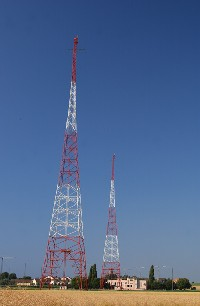
\includegraphics[width=0.8\textwidth]{./images/Analyse/Prangings_VD_CH.jpg}
%  \caption[Zeitzeichensender in Prangins (VD)]{Zeitzeichensender in Prangins (VD) (Quelle: Eigenössisches Institut für Metrologie (METAS); \url{http://www.metas.ch/root_legnet/Web/Fachbereiche/Zeit_Frequenz/dissemination/HBG})} 
%\end{wrapfigure}

\subsection{Zeitzeichensender - DCF77}
DCF77 bezeichnet einen Zeitzeichensender in Deutschland (Mainflingen in Mainhausen) der von der Physikalisch-Technischen Bundesanstalt in Braunschweig (PTB) entwickelt wurde. Der Betrieb erfolgt durch die T-Systems Media Broadcast GmbH, einer Tochtergesellschaft der Deutschen Telekom AG.

%\begin{figure}[H]
%\ffigbox[][7.8cm]{ %
%\begin{subfloatrow}
%  \ffigbox[\FBwidth][]
%    { \caption[Antennenfeld]{Antennenfeld (Quelle: Wikipedia, Patrick Kempf; \url{http://de.wikipedia.org/wiki/DCF77})}}
%    {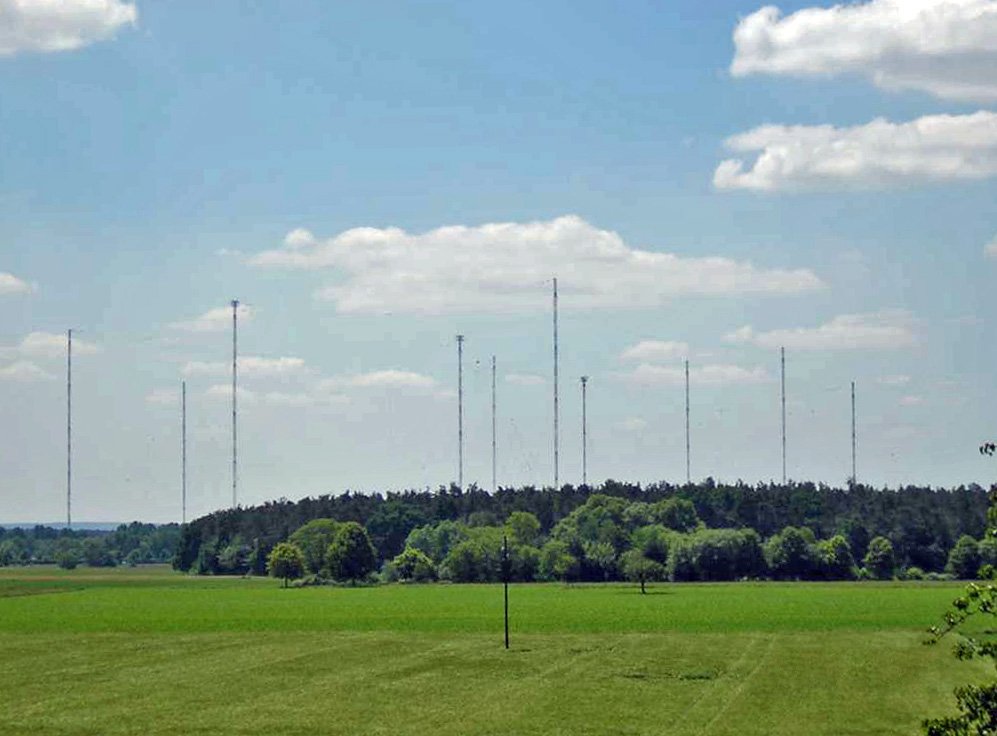
\includegraphics[width=0.5\textwidth]{./images/Analyse/DCF77_Mainflingen.jpg}}
%  \ffigbox[\FBwidth][]
%    {\caption[Sendemast]{Sendemast (Quelle: Physikalisch-Technische Bundesanstalt; \url{http://www.ptb.de/de/aktuelles/archiv/presseinfos/pi2011/pitext/pi111107.htm})} }
%    {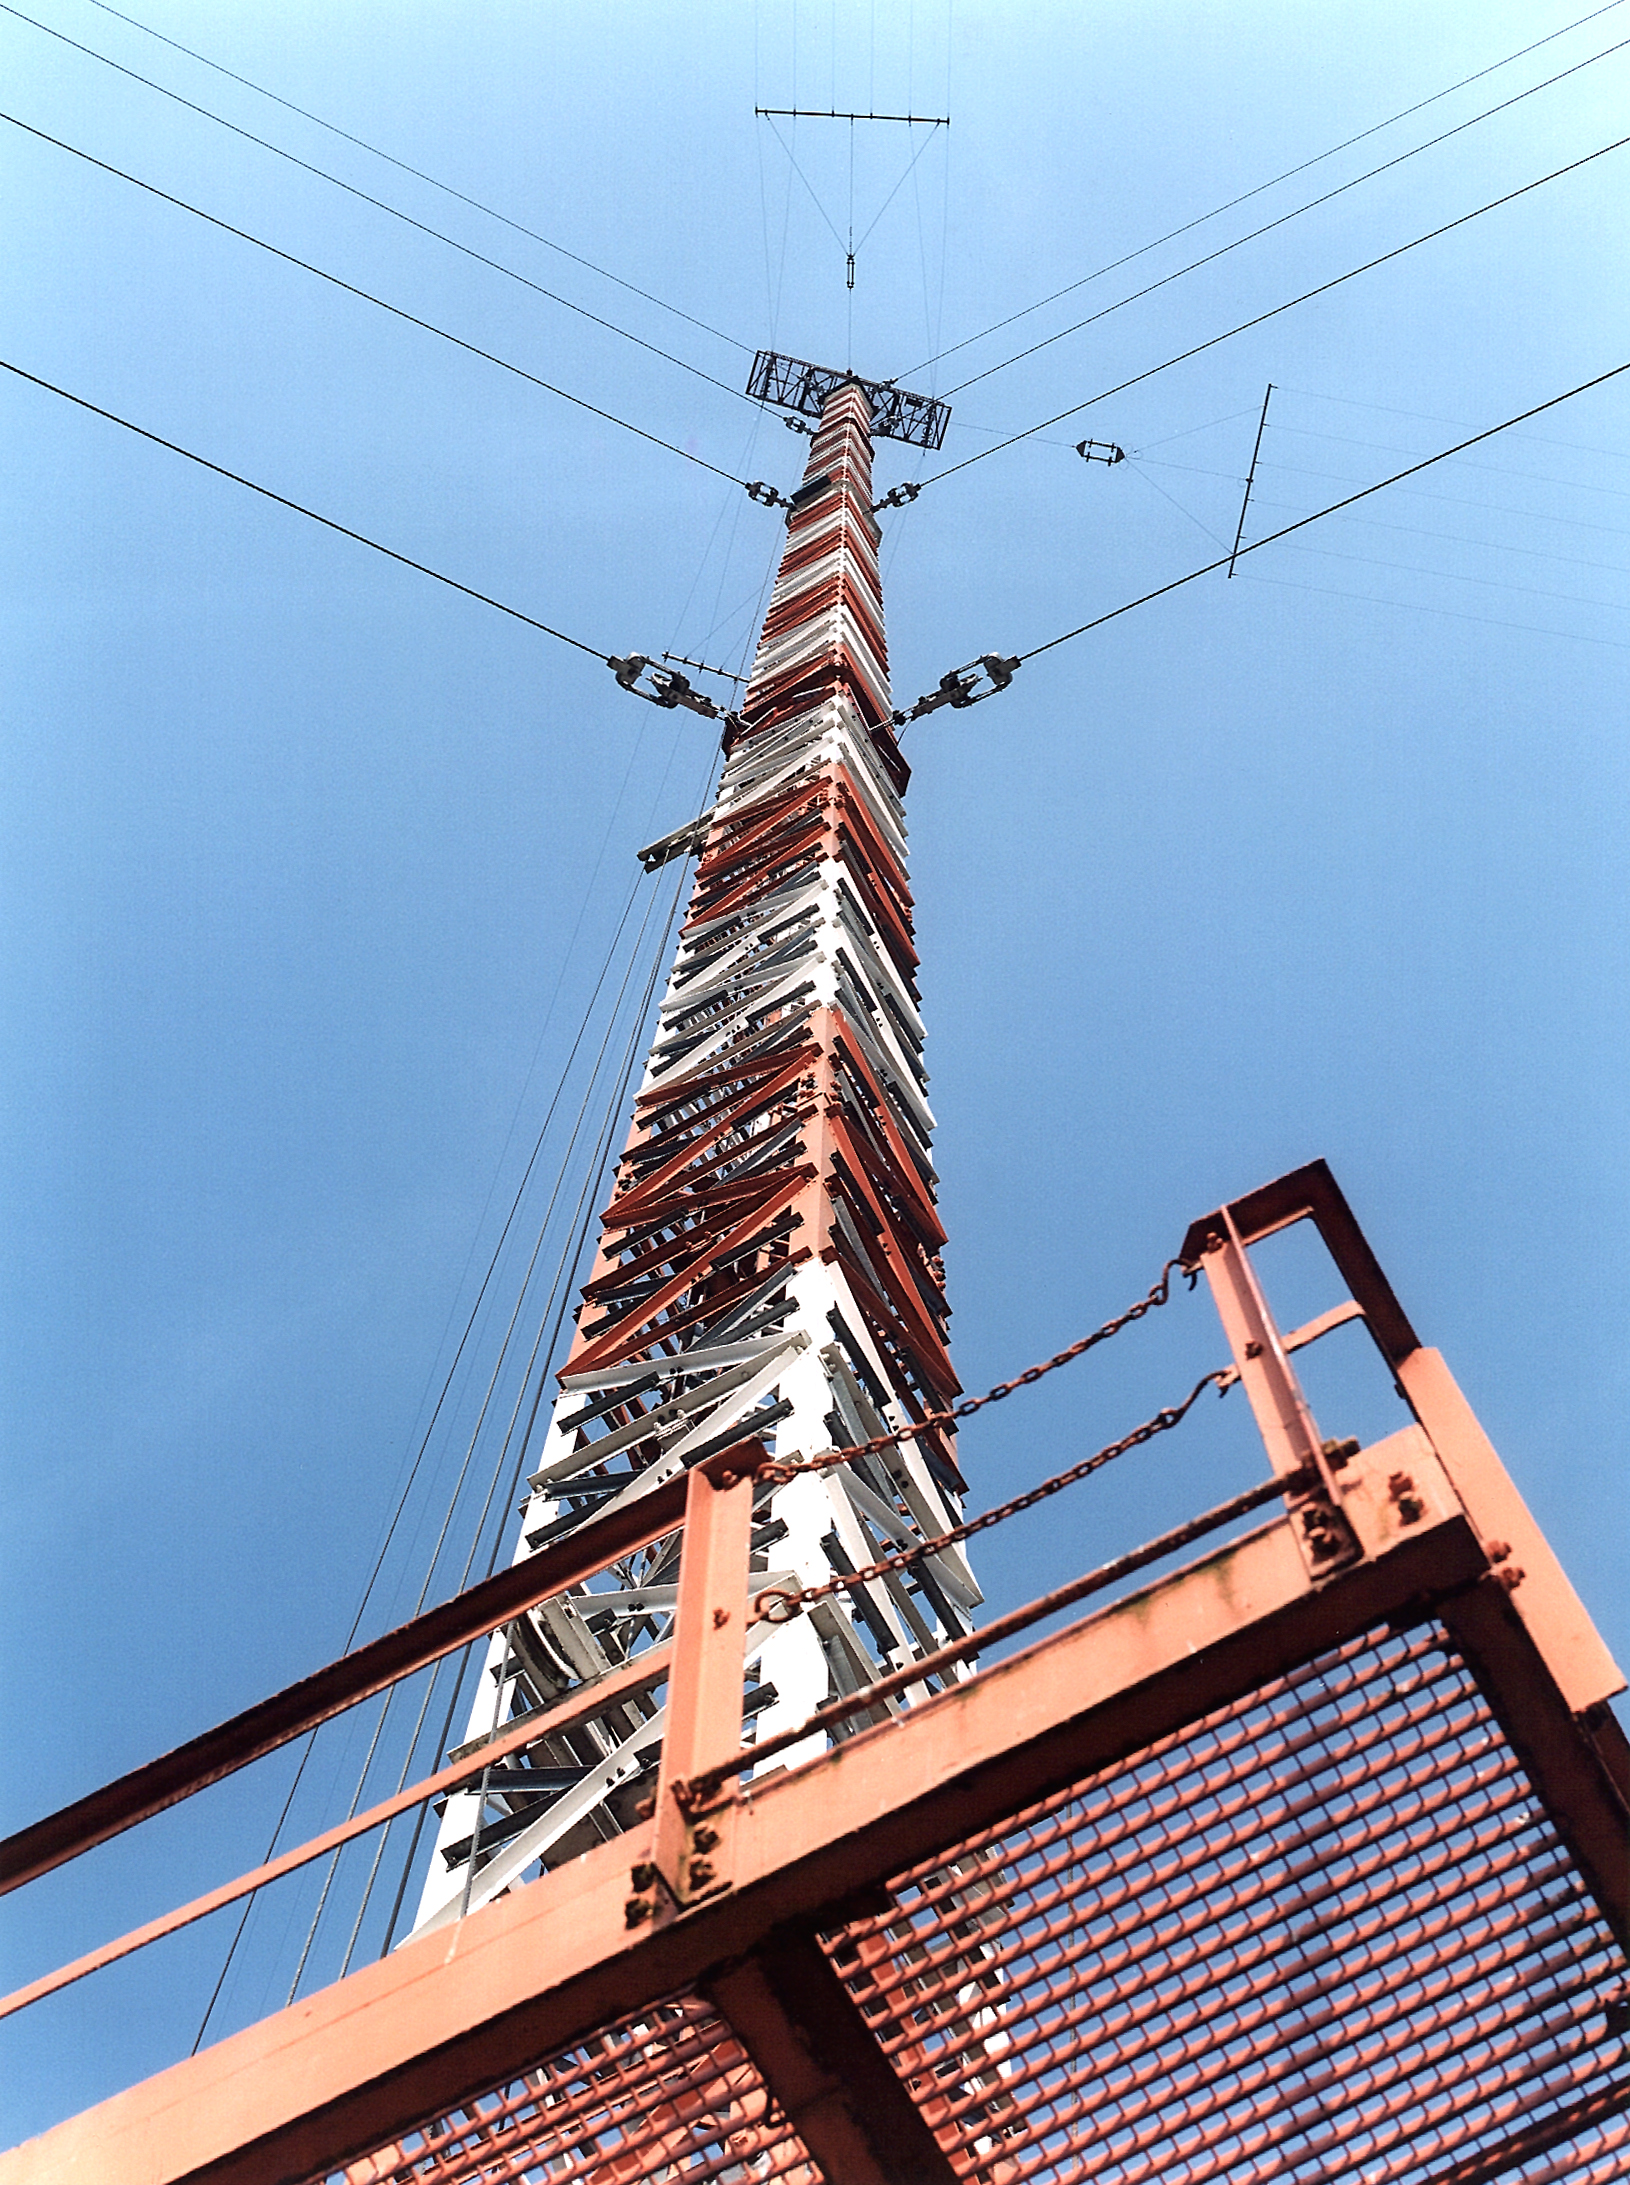
\includegraphics[width=0.5\textwidth]{./images/Analyse/DCF77_Mainflingen_Nah.jpg}}
%\end{subfloatrow}
%}{\caption{Sendeanlage in Mainflingen (Mainhausen, DE)}}
%\end{figure}

\subsubsection{Das Rufzeichen}
Die Bezeichnung setzt sich aus D für Deutschland, C für Langwellensender, F für Frankfurt (Mainhausen liegt in der Nähe von Frankfurt) und 77 für die Sendefrequenz (77.5 kHz). Früher wurde das Rufzeichen des Senders während der 20. bis 32. Sekunde der Minuten 19, 39 und 59 mitgesendet. Es wurde aber festgestellt, dass dies eine Verschlechterung des Signal-zu-Rausch-Abstandes zur Folge hatte. Seither wird das Signal ohne Rufzeichen ausgesendet. Das Signal des DCF77 kann auch ohne Rufzeichen eindeutig identifiziert werden.

\subsubsection{Signalerzeugung}
Das Signal wird von drei unabhängigen Steuereinheiten mit je einer Caesium-Atomuhr erzeugt (1 Hauptkanal, 2 Reservekanäle). Weicht das Signal des Hauptkanals von den Signalen der Reservekanäle ab findet automatische eine Umschaltung auf einen Reservekanal statt. Sind auch diese beiden Signale nicht mehr identisch wird der Vorgang unterbrochen und es wird kein Signal ausgesendet. Jede der drei Einheiten verfügt über eine separate Stromversorgung. Die drei Steuereinheiten sind in einem Speziellen Raum am Sendestandort untergebracht. Darin enthalten ist auch eine weitere Rubidium-Atomuhr, welche als Ersatz und Referenz zur Verfügung steht. Die gesamte Anlage kann via Fernzugriff gesteuert und gewartet werden. 
 
%http://www.hopf.com/de/dcf77-gps_de.html

%\begin{wrapfigure}{r}{0.5\textwidth}
%  \centering
%    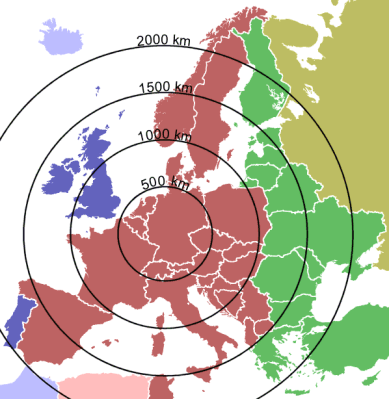
\includegraphics[width=0.5\textwidth]{./images/Analyse/DCF77_Reichweite.png}
%  \caption[Reichweite des Signals]{Reichweite des Signals (Quelle: Compuphase; 
%  \url{http://www.compuphase.com/mp3/h0420_timecode.htm})} 
%\end{wrapfigure}

\subsubsection{Signalreichweite}
Das DCF77 Signal hat je nach Wetterlage, Tages- und Jahreszeit eine Reichweite von 2'000 km. Es wird unterteilt in Bodenwellen, welche sich entlang der Erdoberfläche ausbreiten, und Raumwellen, welche sich durch Reflexion an der ionosphärischen D-Schicht ausbreiten. Bis zu einer Distanz von 500 km vom Sendeort ist die Bodenwelle sehr stabil und überwiegt den Anteil an Raumwellen. Im Bereich von 500 - 1'100 km ist das Verhältnis von Raum- und Bodenwellen etwa gleich gross. Dabei besteht die Gefahr der gegenseitigen Auslöschung. Ab einer Entfernung von 1'100 km nimmt der Anteil an Raumwellen laufend zu.

\subsubsection{Fehleranfälligkeit (Sender \& Empfänger)}
Signale welche mit Amplitudenmodulation können relativ einfach gestört werden, da die Amplitude verhältnismässig leicht von aussen beeinflusst werden kann.

Das Signal kann einerseits unterwegs oder am Empfangsort durch Gewitter, Stürme, Motoren oder elektronische Geräte gestört werden. Andererseits kann auch bereits beim Aussenden des Signals ein Fehler entstehen. Bei heftigen Gewittern, Stürmen oder starken Winden wird die Antenne teilweise vorübergehend ausser Betrieb gesetzt, da durch die Schwingung der Antenne eine messbare Phasenmodulation bei den Empfängern entsteht.

\subsubsection{Genauigkeit}
Das Signal erreicht beim Empfänger, bei optimierter Hardware und optimiertem Decodierungsalgorithmus, eine Genauigkeit von 100 ${\mu}sec$. Bei handelsüblichen Geräten wird jedoch in der Regel nur eine Genauigkeit von 0.1 Sekunden erreicht. Für den Hausgebrauch ist dies vollkommen ausreichend.
In der Industrie ist diese Genauigkeit häufig nicht tragbar.
Durch eine Erhöhung der Bandbreite des Empfängers kann die Abweichung reduziert werden. Dabei wird jedoch auch der Anteil an empfangenen Störsignale grösser. Diese müssen von der Elektronik verarbeitet und ausgefiltert werden.

Für die Bestimmung der Zeit, erreichen die Atomuhren einen relativen Fehler von weniger als $2*10^{-12}$ Sekunden.
Als Referenz dienen dabei die Primären Atomuhren der PTB.
Diese bestimmen die aktuelle Uhrzeit mit einem Fehler zwischen $0.7$ bis $1.2 * 10^{-14}$ Sekunden.
\footnote{Ein Fehler von $10^{-14}$ entspricht ca. einer Milliardstel Sekunde pro Tag ($10^{-14} $) oder einer Sekunde in 2.7 Mio. Jahren.}
%TODO: Review Abweichung, Berechnung ok? - zwar nur halb verstanden aber: SOLVED ;)

\subsubsection{Das Signal}
Seit 1973 wird neben der Normalfrequenz (77.5 kHz) ein digitales Signal gesendet. Das digitale Signal wird durch negative Modulation (Absenkung Trägeramplitude auf 25 \%) auf die Trägerfrequenz aufgebracht und enthält die Informationen zu Datum und Uhrzeit (Mitteleuropäische Zeit, Mitteleuropäische Sommerzeit). Das Signal codiert innerhalb von einer Minute die Zeit- und Datumsinformationen für die darauffolgende Minute.

Der Beginn einer Sekunde (~eines Bits) wird durch die Absenkung der Trägeramplitude markiert. Die Ausnahme bildet hier die letzte Sekunde, bei welcher keine Absenkung statt findet. Je nach Dauer der Amplitudenabsenkung kennzeichnet dies entweder den binären Wert 0 (Absenkung für 100 ms) oder für den Wert 1 (Absenkung für 200 ms).

Das Signal wird anschliessend über einen 50-kW-Halbleitersender ausgesendet. Seit im Jahr 1998 der Halbleitersender in Betrieb genommen wurde dient der vorher verwendete 50-kW-Röhrensender als Ersatz.

\begin{figure}
\ffigbox[][7.8cm]{
\begin{subfloatrow}
  \ffigbox[\FBwidth][]
    {\caption{ohne Amplitudenmodulation}}
    {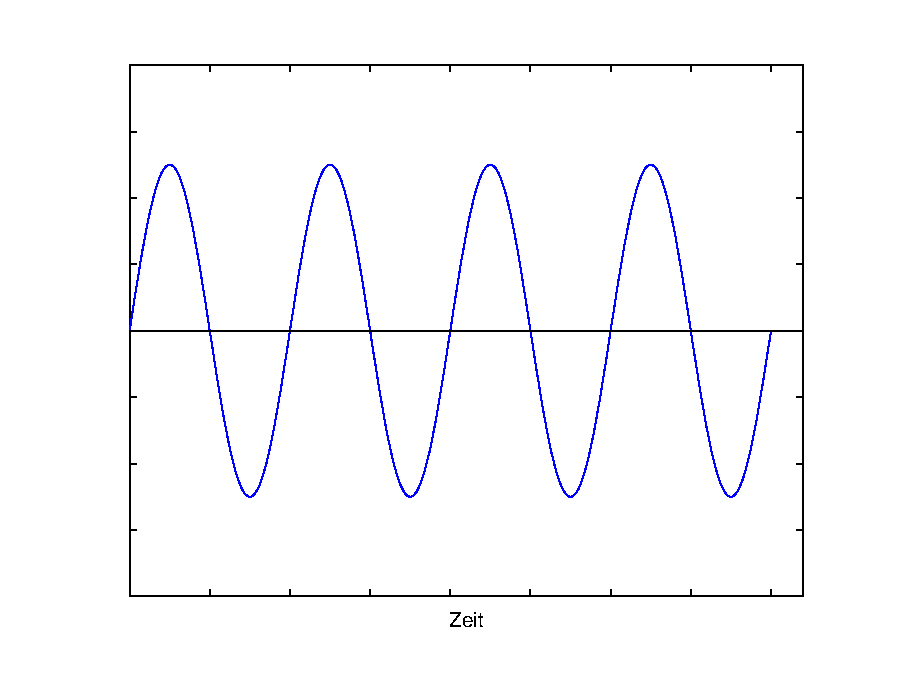
\includegraphics[width=0.5\textwidth]{images/Analyse/SWP2_Analyse_DCF77_Signal_ohne}}
  \ffigbox[\FBwidth][]
    {\caption{mit Amplitudenmodulation}}
    {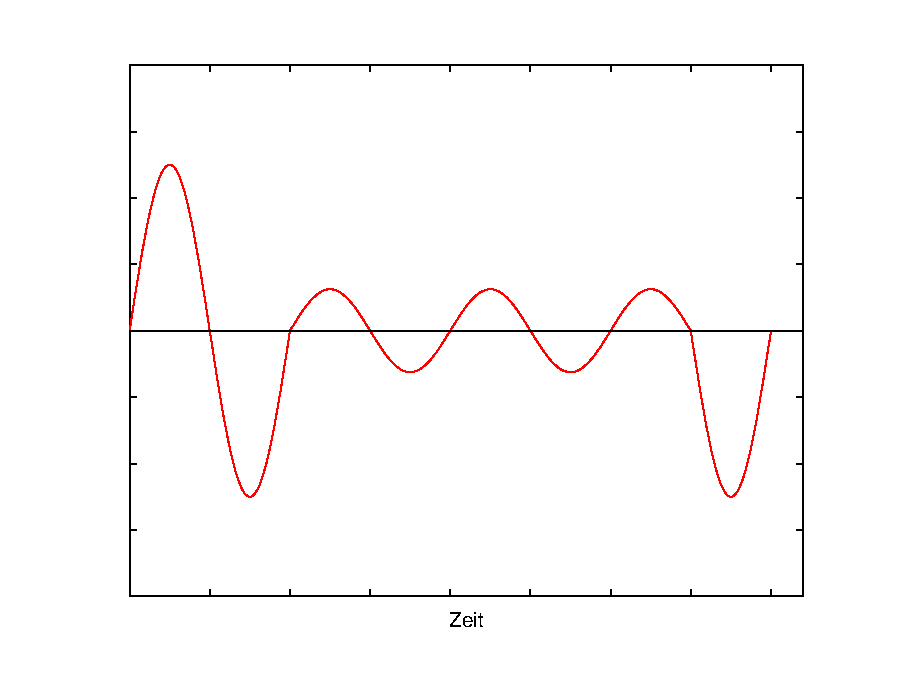
\includegraphics[width=0.5\textwidth]{images/Analyse/SWP2_Analyse_DCF77_Signal_mit}}
\end{subfloatrow}
}{\caption{Beispielhaftes DCF77 Signal}}
\end{figure}

\subsubsection{Codierung}
Die Codierung der Zeitinformation erfolgt anhand der untenstehenden Tabelle.

\begin{itemize}
\item Wochentag: Beginnend bei Montag (1).
\item Monat: Beginnend bei Januar (1).
\item Jahr: Es werden nur die Einer- und Zehnerstellen der Jahreszahl übermittelt (Bsp: 2014, Es wird nur 14 codiert).
\end{itemize}

\newpage

\begin{longtable}{p{1cm} p{13cm}}
\textbf{Bit} & \textbf{Bedeutung} \\ \hline \endhead
0 & Start einer Minute \\
1-14 & Wetterinformationen und Katastrophenschutz \\ \hline
\multicolumn{2}{p{14cm}}{\textit{Informationen zu Unregelmässigkeiten im Sendebetrieb, Zeitzone, Beginn / Ende Sommerzeit, Schaltsekunden}}  \\ \hline
15 & Rufbit \\
16 & Wenn Wert 1: Umstellung MEZ/MESZ am Ende der Stunde \\
17 & Wenn Wert 0: MEZ, Wenn Wert 1: MESZ \\
18 & Wenn Wert 0: MESZ, Wenn Wert 1: MEZ \\
19 & Wenn Wert 1: Schaltsekunde am Ende der Stunde. \\ \hline
\multicolumn{2}{p{14cm}}{\textit{Zeitinformation der nachfolgenden Minute in BCD-Zahlen (Start mit LSB). Gerade Parität für Fehlererkennung.}}  \\ \hline
20 & Beginn der Zeitinformation (immer 1) \\
21 & Minute (Einer) - Bit für 1 \\
22 & Minute (Einer) - Bit für 2 \\
23 & Minute (Einer) - Bit für 4 \\
24 & Minute (Einer) - Bit für 8 \\
25 & Minute (Zehner) - Bit für 10 \\
26 & Minute (Zehner) - Bit für 20 \\
27 & Minute (Zehner) - Bit für 40 \\
28 & Parität Minute \\ \hline
29 & Stunde (Einer) - Bit für 1 \\
30 & Stunde (Einer) - Bit für 2 \\
31 & Stunde (Einer) - Bit für 4 \\
32 & Stunde (Einer) - Bit für 8 \\
33 & Stunde (Zehner) - Bit für 10 \\
34 & Stunde (Zehner) - Bit für 20 \\
35 & Parität Stunde \\ \hline
36 & Kalendertag (Einer) - Bit für 1 \\
37 & Kalendertag (Einer) - Bit für 2 \\
38 & Kalendertag (Einer) - Bit für 4 \\
39 & Kalendertag (Einer) - Bit für 8 \\
40 & Kalendertag (Zehner) - Bit für 10 \\
41 & Kalendertag (Zehner) - Bit für 20 \\
42 & Wochentag - Bit für 1 \\
43 & Wochentag - Bit für 2 \\
44 & Wochentag - Bit für 4 \\
45 & Monatsnummer (Einer) - Bit für 1 \\
46 & Monatsnummer (Einer) - Bit für 2 \\
47 & Monatsnummer (Einer) - Bit für 4 \\
48 & Monatsnummer (Einer) - Bit für 8 \\
49 & Monatsnummer (Zehner) - Bit für 10 \\
50 & Jahr (Einer) - Bit für 1 \\
51 & Jahr (Einer) - Bit für 2 \\
52 & Jahr (Einer) - Bit für 4 \\
53 & Jahr (Einer) - Bit für 8 \\
54 & Jahr (Zehner) - Bit für 10 \\
55 & Jahr (Zehner) - Bit für 20 \\
56 & Jahr (Zehner) - Bit für 40 \\
57 & Jahr (Zehner) - Bit für 80 \\
58 & Parität Datum \\
59 & Keine Sekundenmarke
\end{longtable}

Idealerweise sollte ein Gerät das Signal mindestens zwei Minuten ungestört empfangen können um die Zeit eindeutig einzustellen. Auf jeden Fall werden die ersten 36 Sekunden und anschliessend ein Minutenübergang (Sekunden 58 und 59) benötigt.

\begin{wrapfigure}{r}{\textwidth}
  \begin{center}
    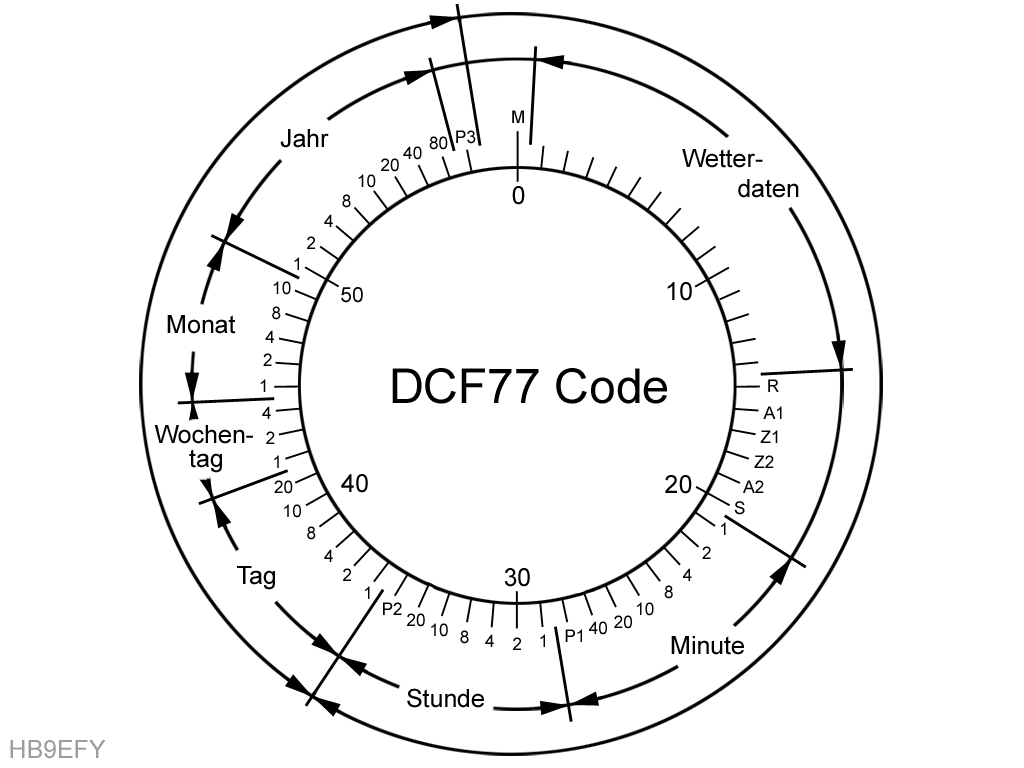
\includegraphics[width=\textwidth]{./images/Analyse/DCF77_Codierscheibe.png}
  \end{center}
  \caption[DCF77-Codierung als Codierscheibe]{DCF77-Codierung als Codierscheibe (Quelle: Endorphino; 
  \url{http://endorphino.de/projects/electronics/timemanipulator/index.html})} 
\end{wrapfigure}

\begin{landscape}
Die Zeitangabe "`12.03.2014 18:15:30"' (MEZ) wird wie folgt als DCF77-Signal codiert:\\\\
\begin{tabular}{r | c c c c c c c c c c c c c c c c c c c c}
\multicolumn{20}{c}{}	\\
Bitnr.	 &	0	&	1	& 	2	&	3	&	4	&	5	&	6	&	7	&	8	&	9	&	10	&	11	&	12	&	13	&	14	&	15	&	16	&	17	&	18	&	19	\\
Wert	&	0	&	0	& 	0	&	0	&	0	&	0	&	0	&	0	&	0	&	0	&	0	&	0	&	0	&	0	&	0	&	0	&	0	&	0	&	1	&	0	\\
\\\hline \\
	&  	&\multicolumn{7}{| c |}{\textit{Minute: 30}}	&	\multicolumn{6}{c |}{\textit{Stunde: 18}}	&	\multicolumn{4}{c }{\textit{Kalendertag: 12}}	\\
Bitnr.	&	20	&	21	&	22	&	23	&	24	&	25	&	26	&	27	&	28	&	29	&	30	&	31	&	32	&	33	&	34	&	35	&	36	&	37	&	38	&	39	\\
Wert	&	1	&	0	&	0	&	0	&	0	&	1	&	1	&	0	&	0	&	0	&	0	&	0	&	1	&	1	&	0	&	0	&	0	&	1	&	0	&	0	\\
\\\hline \\
	&   \multicolumn{2}{ c |}{}	& \multicolumn{3}{ c |}{\textit{Wochentag: MI}}	&	\multicolumn{5}{ c |}{\textit{Monat: März}}	&		\multicolumn{8}{ c |}{\textit{Jahr: 2014}}	&		&		\\
Bitnr.	&	40	&	41	&	42	&	43	&	44	&	45	&	46	&	47	&	48	&	49	&	50	&	51	&	52	&	53	&	54	&	55	&	56	&	57	&	58	&	59	\\
Wert	&	1	&	0	&	1	&	1	&	0	&	1	&	1	&	0	&	0	&	0	&	0	&	1	&	1	&	1	&	0	&	0	&	0	&	0	&	0	&	-
\end{tabular}

%TODO: zweites Beispiel (Evtl. Wechsel Sommerzeit)
%TODO: Evtl. Zeile mit BCD-Wertigkeit?
\end{landscape}

\subsubsection{BCD-Codierung}
Kurz zur verwendeten BCD-Codierung (Binary Coded Decimal):\\
Jede Ziffer einer Zahl wird einzeln mit 4 Bit (8, 4, 2, 1) codiert. Von den $2^4 = 16$ Kombinationsmöglichkeiten werden nur 10 verwendet, darum spricht man oft von einer Speicherverschwendung.

\subsubsection{Zusatznutzung}
Das Signal des Zeitzeichensenders wird seit Ende 2006 zusätzlich für Alarmierungen und Wetterdaten eingesetzt. Dafür werden die ersten 14. Bit der Minute verwendet. Im Katastrophenfall werden Details zur Katastrophe und der Region übermittelt. Diese Informationen werden aufgrund ihrer Auswirkungen doppelt gesichert (Paritätsbit und Wiederholung). Die Wetterdaten werden von der Firma Meteo Time GmbH bereitgestellt und ermöglichen eine viertägige Vorhersage für 60 Regionen in Europe. Die Decodierung dieser Wetterdaten ist jedoch lizenzpflichtig da diese im proprietären Meteo-Time-Protokoll übermittelt werden.

\subsection{Fehlererkennung beim Empfänger}
In die Codierung ist eine einfache Fehlererkennung, anhand einer einfachen Parität, eingebaut. Die Fehlererkennung ist jedoch bei Blockfehlern und Fehlermaskierung nicht immer gewährleistet. In der Praxis wird häufig auf Redundanz, bzw. Stetigkeit und Kontinuität der gelieferten Zeitinformationen gesetzt.

Dazu ein Beispiel:\\
In den aktuellen Zeitinformationen wird das Jahr 2014 und der Monat März geliefert. In den vorangehenden Minuten / Stunden wurde aber immer das Jahr 2014 und der Monat Januar geliefert. Daraus lässt sich schliessen, dass es sich bei der aktuellen Zeitinformation um einen Fehler handelt.

Eine Fehlerkorrektur ist mit einer einfachen Parität nicht möglich. Werden jedoch die Daten der letzten Minute / Stunde / Tag hinzugezogen kann basierend auf dem Inhalt eine Fehlerkorrektur durchgeführt werden.

\subsection{Fehlererkennung beim Sender}
Das in Mainflingen ausgesendete Signal wird an Braunschweig ausgewertet, analysiert und bei Bedarf ein Alarm ausgelöst. Der Alarm wird ausgelöst, wenn während mehrerer Minuten die gleichen logischen Fehler im Signal erkannt wurden oder wenn auf technischer Ebene eine Unregelmässigkeit festgestellt wurde (z.B. zu kleines Signal über eine längere Zeitdauer).

\subsubsection{Network Time Protocol}
Wird bei eine NTP-Root-Server (Siehe Kapitel \ref{Anaylse:Internet}) das DCF77-Signal als Referenz verwendet wird dieser mit der Kennung "`.DCFa"' gekennzeichnet.

\subsection{GPS}
Nebst der Zeitsynchronisation über Funk, kann eine genauere Information von den GPS-Satelliten gewonnen werden. Dies obwhol GPS-Systeme hauptsächlich zur Lokalisierung des Standortes entwickelt wurden.
Momentan befinden sich sechs solche Satelliten auf ungefähr 200'000 km Höhe. Jeder umrundet die Erde zweimal pro Tag. Auf jedem Satellit sind jeweils zwei Atomuhren vorhanden.
Ein Satellit sendet andauernd seine Bahnposition und die genaue Uhrzeit. Durch Signale mehrerer Satelliten, kann der Empfänger seinen genauen Standort berechnen.
Anschliessend kann die Laufzeit des Signals zurück gerechnet und die durchs Versenden verstrichene Zeit, der Delay, approximiert werden.
Durch dieses Verfahren kann die Uhrzeit mit einer Genauigkeit unter 1 ${\mu}sec$ berechnet werden.

Vorteile der Zeit-Synchronisation über GPS sind die weltweite Abdeckung und eine höhere Genauigkeit als die Synchronisation über Zeitzeichensender.

Ein grosser Nachteile der GPS Synchronisation ergibt sich jedoch durch das verwendete Kurzwellen Signal (zwischen 1176,45 bis 1575,42 MHz). Dieses Signal kann parktisch nur unter freien Himmel empfangen werden und eignet sich daher nicht für einen typischen Computer.

%GPS: http://www.mono.rgbtechnology.pl/de/faq/gps-zeitsynchronisation.html
%http://www.stardado.de/1244, http://www.emsec.rub.de/media/crypto/attachments/files/2010/04/ms_michael_ziaja.pdf
%GPS vs DCF77: http://www.hopf.com/de/dcf77-gps_de.html
\subsection{Internet} \label{Anaylse:Internet}

Will man eine Uhr via Internet synchronisieren, stösst man auf folgendes Problem:

\begin{verse}
Die genaue Sendedauer eines  Datenpaktes, welches die korrekete Uhrzeit beinhaltet, ist weder vorhersehbar, noch kan man die verstrichene Zeit beim Empfänger zurückrechnen.
\end{verse}

Da keine Aussage über die Genauigkeit der empfangenen Information möglich ist, verliert sie drastisch an Wert.

%TODO: Evtl. Kapitel NTP vorziehen -> Verständnis
\section{Zeitprotokoll}
Um eine brauchbare Synchronisation via Internet zu ermöglichen wurde folgender, vereinfachter Datenaustausch definiert: (Der Client synchronisiert seine Zeit mit der genauen Zeit eines Server. Die Serverzeit entspricht also nicht der Clientzeit.)\cite{stackoverflowNtp}



\begin{enumerate}
\item Der Client schickt eine \textbf{Anfrage an den Server} und \textbf{merkt} sich seine aktuelle, lokale Zeit (welche mit grosser Wahrscheinlichkit nicht der korrekten Serverzeit entspricht).
\item Der Server antwortet mit seiner lokalen, korrekten \textbf{Zeit des Empfangs und der des (geplanten) Rückversandes}.
\item Der Client merkt sich die Empfangszeit der Antwort. 
\end{enumerate}
\vspace{1em}
Nach dem Datenaustausch hat der Client folgende vier verschiedene Zeiten zur Verfügung:
\begin{enumerate}
\item Client: lokale Zeit der Anfrage - (A)
\item Server: Empfangszeit - (X)
\item Server: Versandzeit - (Y)
\item Client: Empfangszeit - (B)
\end{enumerate}
\vspace{1em}
Als Annahme wird vereinfacht angenommen, das der Hinweg des Paketes ungefähr gleich lang wie der Rückweg dauert.
\vspace{1em}
Nun kann der Client mit folgender Rechnung die Uhrzeit gut annähern (inkl. der dazugehörigen Fehlerabschätzung):
\begin{itemize}
\item Totale Zeit des Prozesses: B-A
\item Server Bearbeitungszeit: Y-X
\item Effektive Datentransferzeit: B-A-(Y-X)
\item Datentransferzeit Rückweg: [B-A-(Y-X)]/2
\item Korrekte Zeit; plus dauer des Rückweges: Y+[(B-A-(Y-X))/2]
\item als Fehlerabschätzung wird die Hälfte der \textit{Effektive Datentransferzeit} verwendet: B-A-(Y-X)
\end{itemize}

\subsubsection{Beispiel Synchronisation}
Ein konkretes Beispiel dazu (Zur Vereinfachung in Milisekunden).\\
\vspace{0em}
(Die Clientzeit ist jeweils falsch. Die Serverzeit ist korrekt. Die zwei Zeiten sind nicht synchron und dürfen daher nicht direkt miteinander verrechnet werden.)
\begin{itemize}
\item Clientzeit lokal beim Senden: A = 200
\item Serverzeit des Empfangs: X = 150
\item Serverzeit Rückversand: Y = 180
\item Clientzeit Empfang: B = 300
\end{itemize}

Daraus kann auf folgendes gschlossen werden:
\begin{itemize}
\item Totale Zeit des Prozesses: B-A = 300-200 = \textbf{100}
\item Server Bearbeitungszeit: Y-X = 180-150 = \textbf{30}
\item Effektive Datentransferzeit: [B-A]-([Y-X]) = 100 - 30 = \textbf{70}
\item Nur Rückweg: (B-A-(Y-X))/2 = 70/2 = \textbf{35}
\item Korrekte Zeit, plus dauer des Rückweges: Y+[(B-A-(Y-X)/2)] = 180+35 = \textbf{215}
\item Feherabschätzung: max. 35\\
Das Worstcase Szenario ist folgendes:\\
\begin{itemize}
\item Client $\Rightarrow$ Server: $\approx$0
\item Server $\Rightarrow$ Client:$ \approx$70
\end{itemize}
$\Rightarrow$ \textbf{Fehler: 35},
\end{itemize}

\section{NTP / SNTP}
NTP (Network Time Protocol) basiert auf dem oben beschriebenen Prinzip, hat aber noch diverse Verbesserungen in sich.
NTP befindet sich momentan in der Version 4.
Da das Protokoll sehr komplex ist, gibt es auch eine vereinfachte Version, die SNTP (Simple Network Time Protocol) genannt wird.
Die genaue Funktionsweise dieses Protokolles wird in dieser Arbeit nicht erläutert.

%TODO: Isch etzte s Bispiel obe SNTP oder no e witer Vereifachti Form?
% http://www.eecis.udel.edu/~mills/database/reports/ntp4/ntp4.pdf
% http://www.emsec.rub.de/media/crypto/attachments/files/2010/04/ms_michael_ziaja.pdf

\section{Weitere Zeitsignaldienste}
Es gibt einige weitere Zeitsignaldienste, welche jedoch in der heutigen Zeit keine grosse Bedeutung mehr haben. Das Zeitsignal wird zum Teil auch als Zusatzinformation auf dem Hörfunk oder im Video- / Teletext von Fernsehsendern übertragen. Früher wurde auch über das öffentliche Telefon eine Zeitdienst angeboten.

\section{Fazit}
Mit Hilfe der Analyse konnten nachfolgend im Detail beschriebene Schwerpunkte und Herausforderungen für die Umsetzung des Projektes identifiziert werden.

\subsection{Codierung der Zeitinformationen einer Minute}
Da während einer Minute die Zeitinformationen der nächsten Minute codiert wird stehen jeweils nur zum Minutenübergang zur Verfügung. Während der Minute müssen die Sekunden, bzw. die Sekundenkennungen, gezählt werden um die aktuelle Zeit zu ermitteln. Daraus folgt, dass eine eigenständige Uhr implementiert werden muss die mit diesen Gegebenheiten umgehen kann. Zum einen muss die Uhr komplett ohne das Signal auskommen und akkurat weiterlaufen und zum anderen muss bei Empfang der Sekunden- und Minutenkennungen entsprechend reagiert und die Uhr justiert werden. 

Die Implementation dieser Uhr wird nicht einfach werden, da wir uns nur auf Informationen verlassen können, die direkt von der Hardware kommen. Wenn z.B. eine Sekunde mit einer gewissen Anzahl Durchläufe in einer Schleife angenähert wird, ist nicht garantiert, dass diese immer gleich lange dauert. Grund dafür ist, dass auch andere Prozesse und Threads CPU-Zeit erhalten. Eine weitere Herausforderung wird es sein, die Implementation so Systemnah wie möglich zu halten um die Verarbeitungszeit und die resultierende Ungenauigkeit zu minimieren.

\subsection{Fehlererkennung und Fehlerkorrektur}
Die Wellen, bzw. das Signal des DCF77 können aufgrund ihrer Eigenschaften relativ leicht gestört werden. Aufgrund dessen muss unsere Implementation in der Lage sein fehlerhafte Informationen zu erkennen und zu korrigieren. Dafür muss das "`Langzeitverhalten"' gespeichert, analysiert und entsprechend reagiert werden. Dabei muss beachtet werden, dass zunächst als Fehler erkannte Informationen auch keine Fehler sein können. Wird z.B. bei der Umstellung Winter- / Sommerzeit eine Stunde im Voraus das entsprechende Bit gesetzt muss dieses korrekt interpretiert werden und darf nicht über die gesamte Stunde als Fehler herausgefiltert werden. Wird eine Information über längere Zeit übermittelt ist muss diese nach einer gewissen Zeit als richtig erkannt werden.


